% LINGI2255 - Software Development Project
% Manual
\documentclass{article}
\usepackage[utf8]{inputenc}
\usepackage[UKenglish]{babel}
\usepackage{graphicx}

\title{Manual}


\usepackage{caption}% http://ctan.org/pkg/caption
\captionsetup[figure]{labelformat=empty}%

\begin{document}

\section{Introduction}
We will together discover the various features of the site Care4Care.

In the various screenshots, the left mouse button is represented by a red dot. 

\section{Sign in}
\begin{figure}[!ht]
   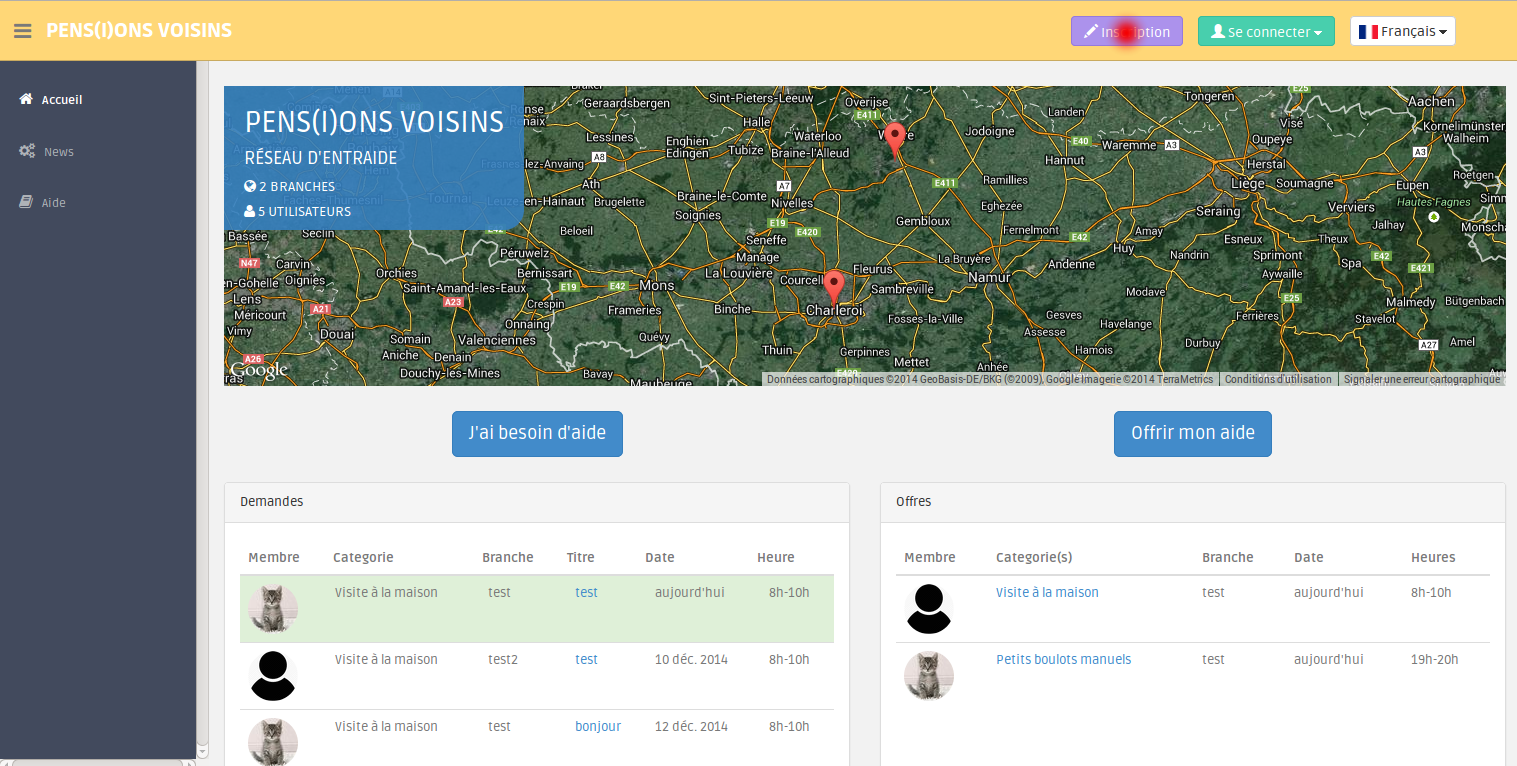
\includegraphics[width=\textwidth]{img/inscr1.png}
   \caption{Sign in: Step 1}
\end{figure}

\begin{figure}[!ht]
   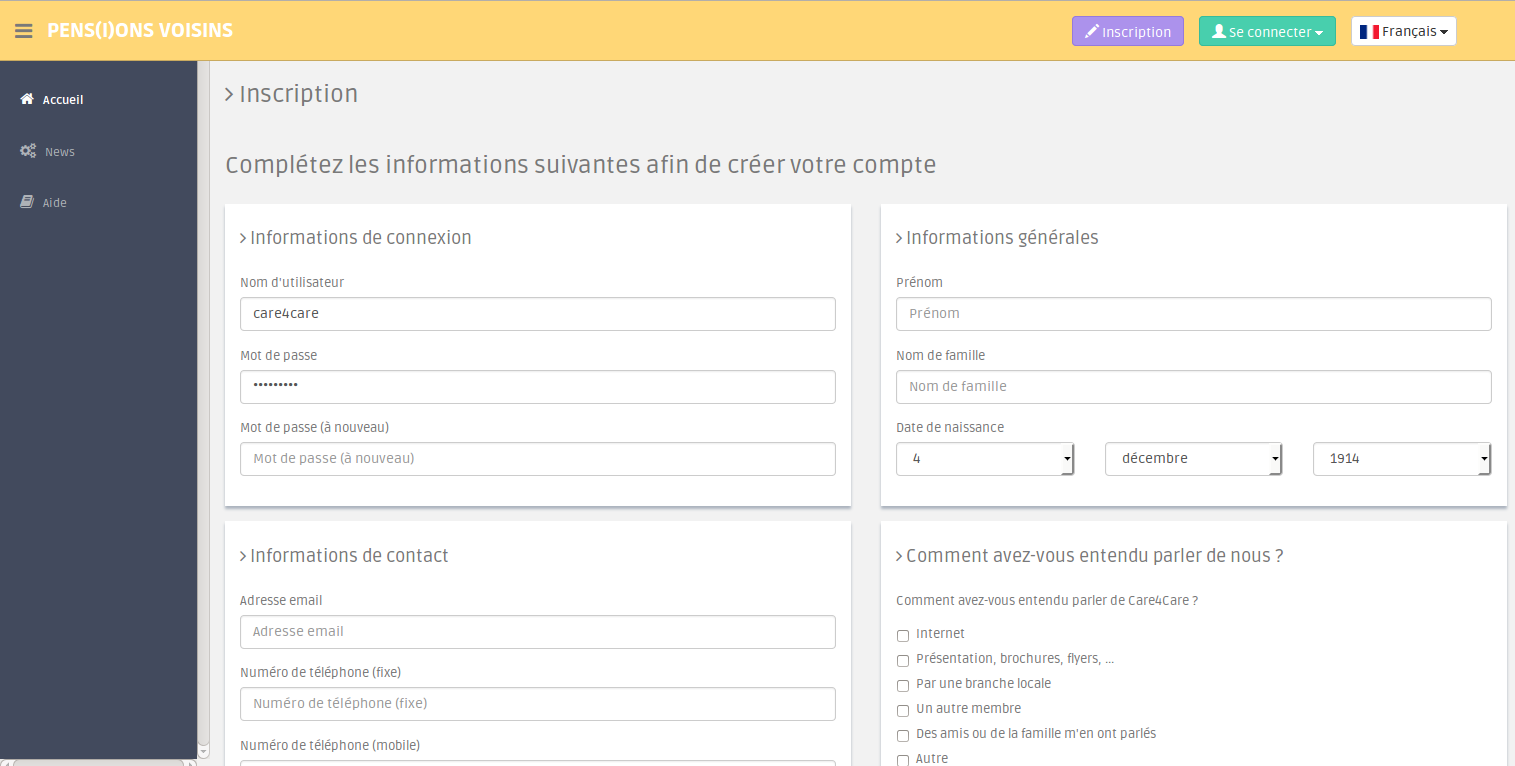
\includegraphics[width=\textwidth]{img/inscr2.png}
   \caption{Sign in: Step 2 - Fill in this form}
\end{figure}

\begin{figure}[!ht]
   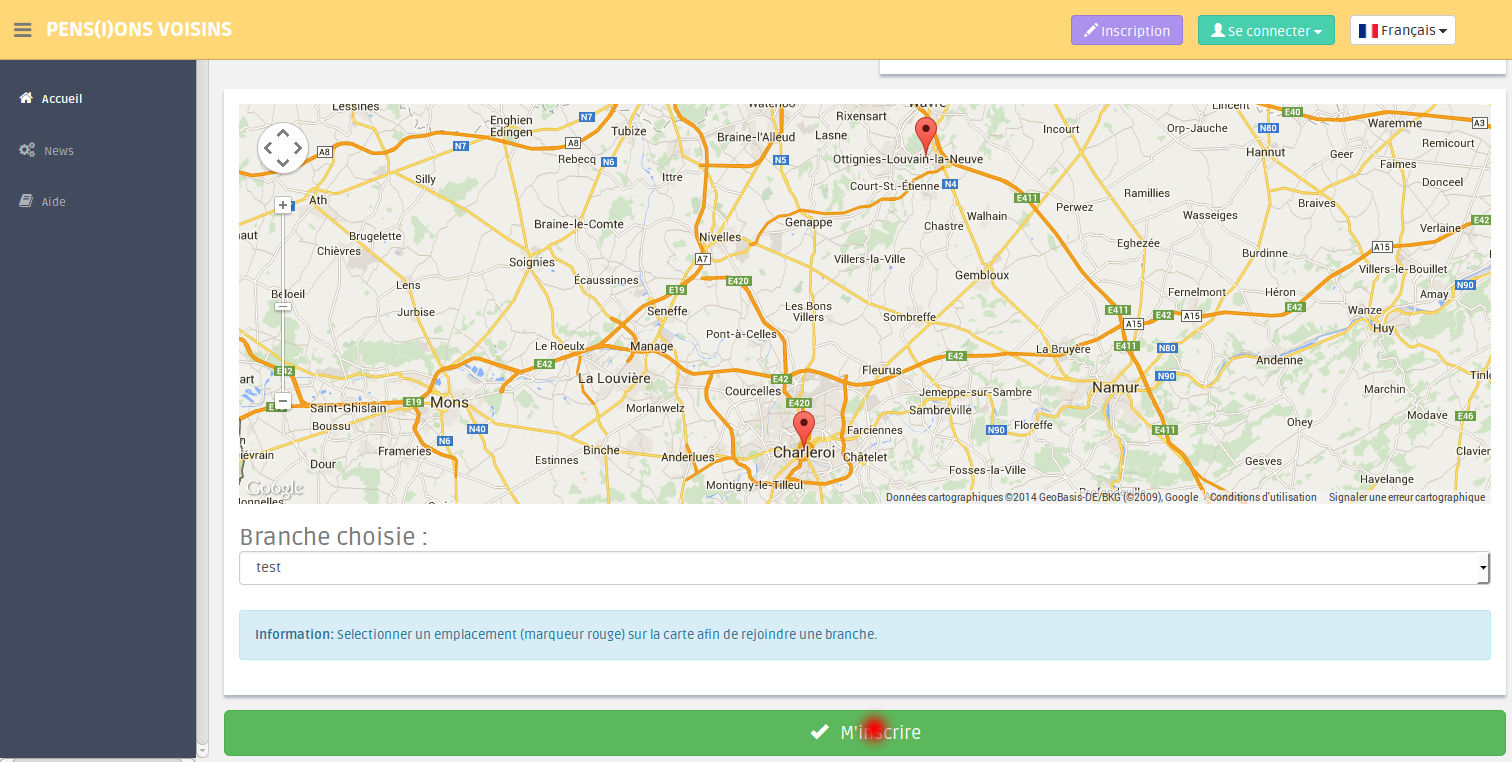
\includegraphics[width=\textwidth]{img/inscr3.png}
   \caption{Sign in: Step 3 - Send demand}
\end{figure}

\clearpage
\section{Display the menu}
\begin{figure}[!ht]
   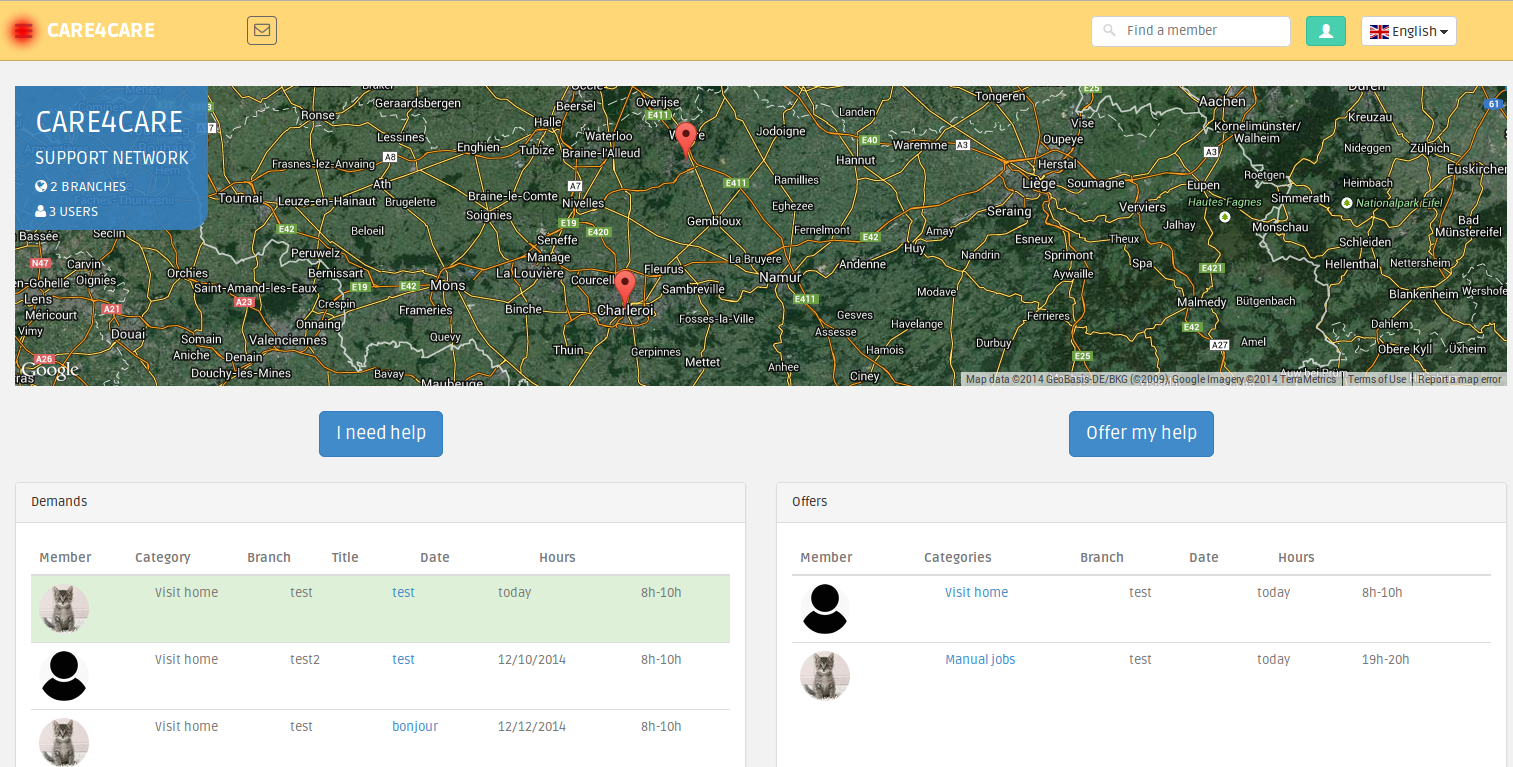
\includegraphics[width=\textwidth]{img/menu1.png}
   \caption{Menu: Step 1}
\end{figure}
\begin{figure}[!ht]
   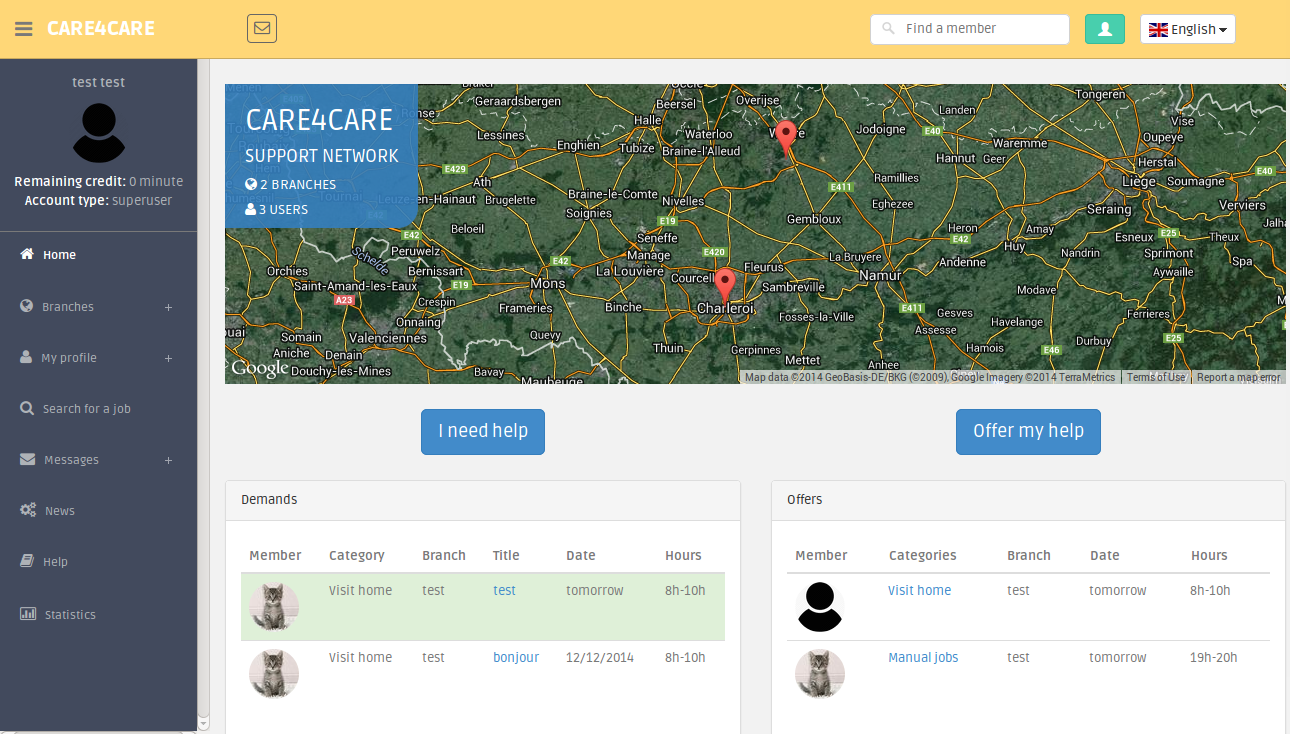
\includegraphics[width=\textwidth]{img/menu2.png}
   \caption{Menu: Result}
\end{figure}

\clearpage
\section{Sign out}
\begin{figure}[!ht]
   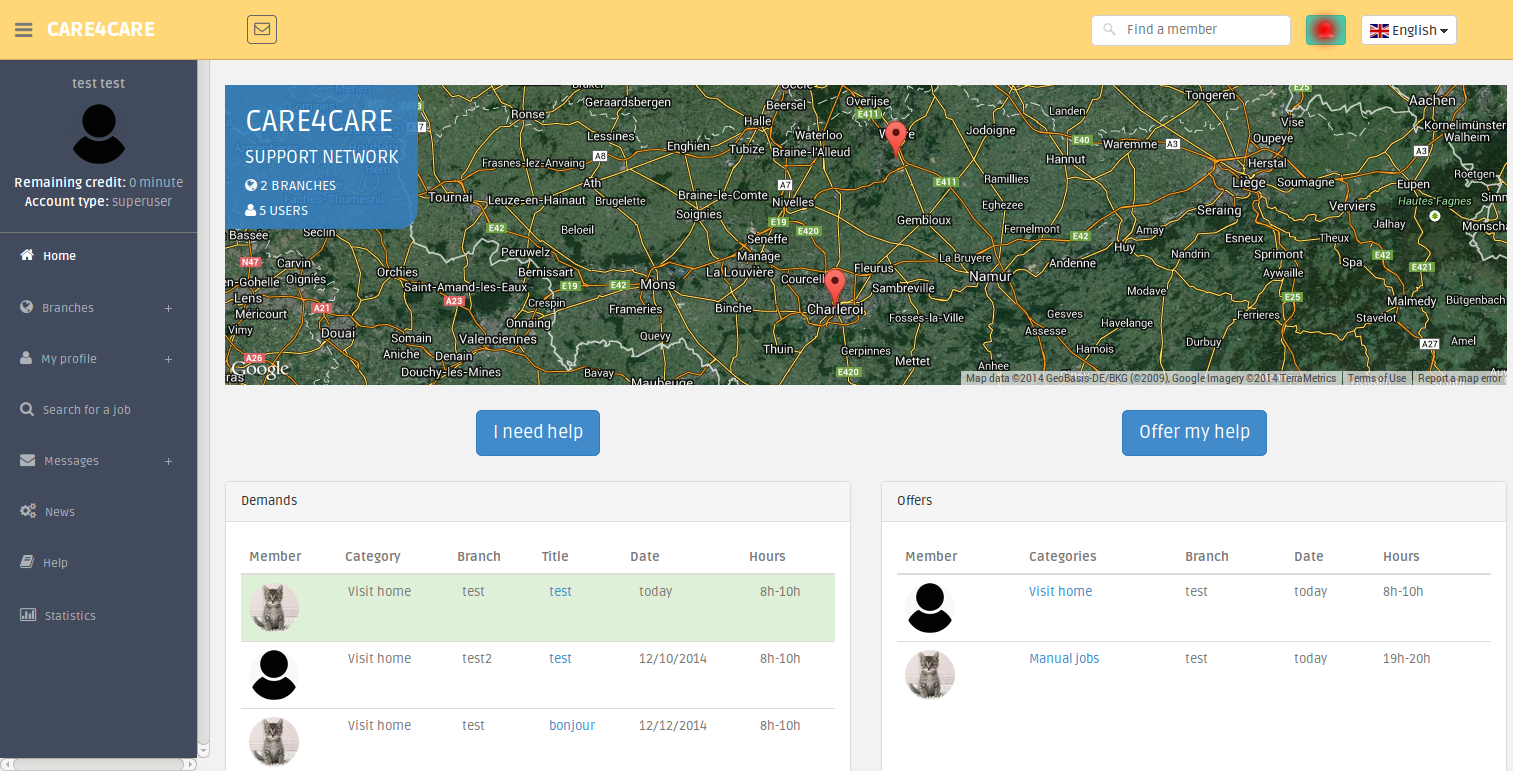
\includegraphics[width=\textwidth]{img/out1.png}
   \caption{Sign out: Step 1}
\end{figure}
\begin{figure}[!ht]
   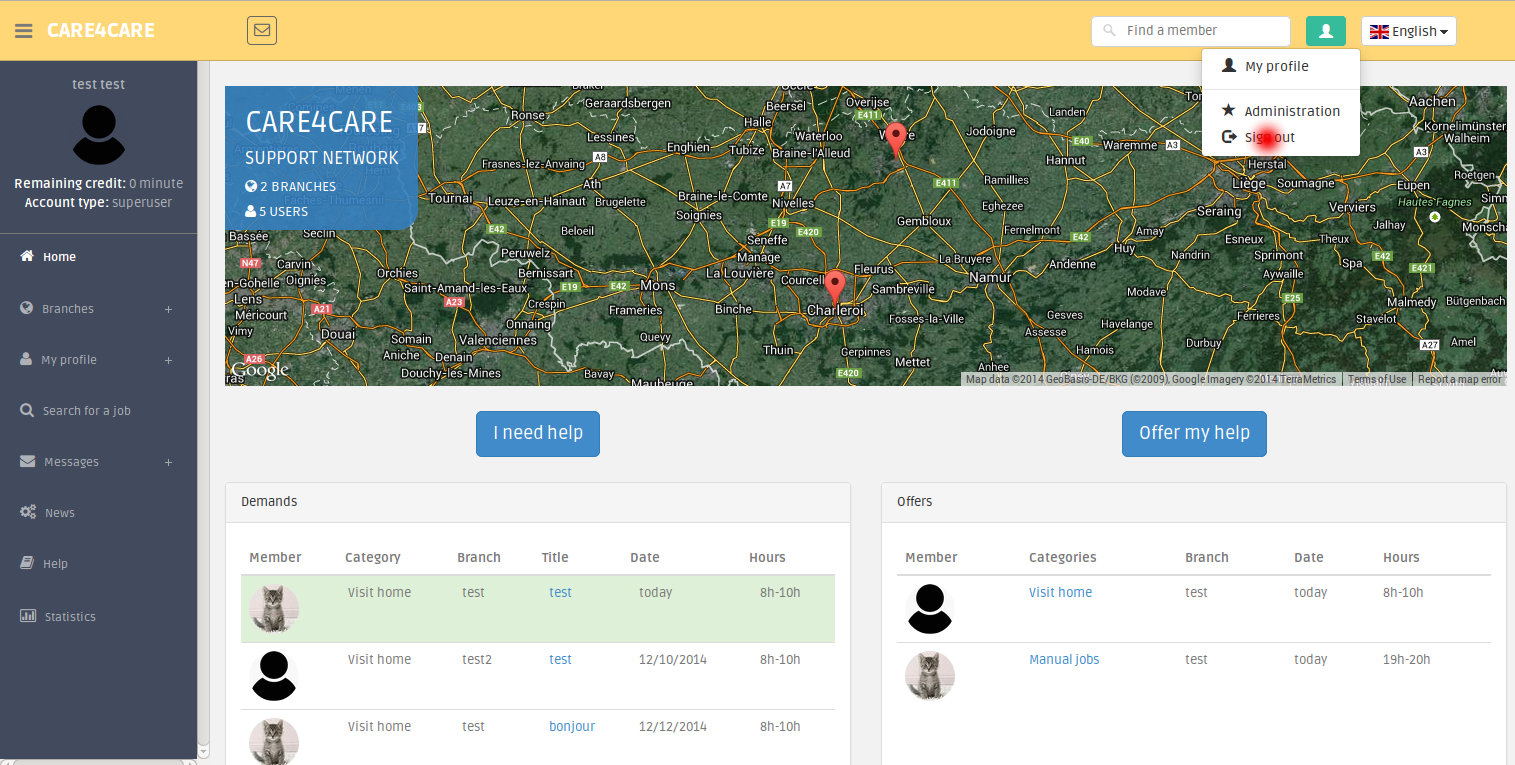
\includegraphics[width=\textwidth]{img/out2.png}
   \caption{Sign out: Step 2}
\end{figure}

\clearpage
\section{My profil}
\subsection{Display my profil}
\begin{figure}[!ht]
   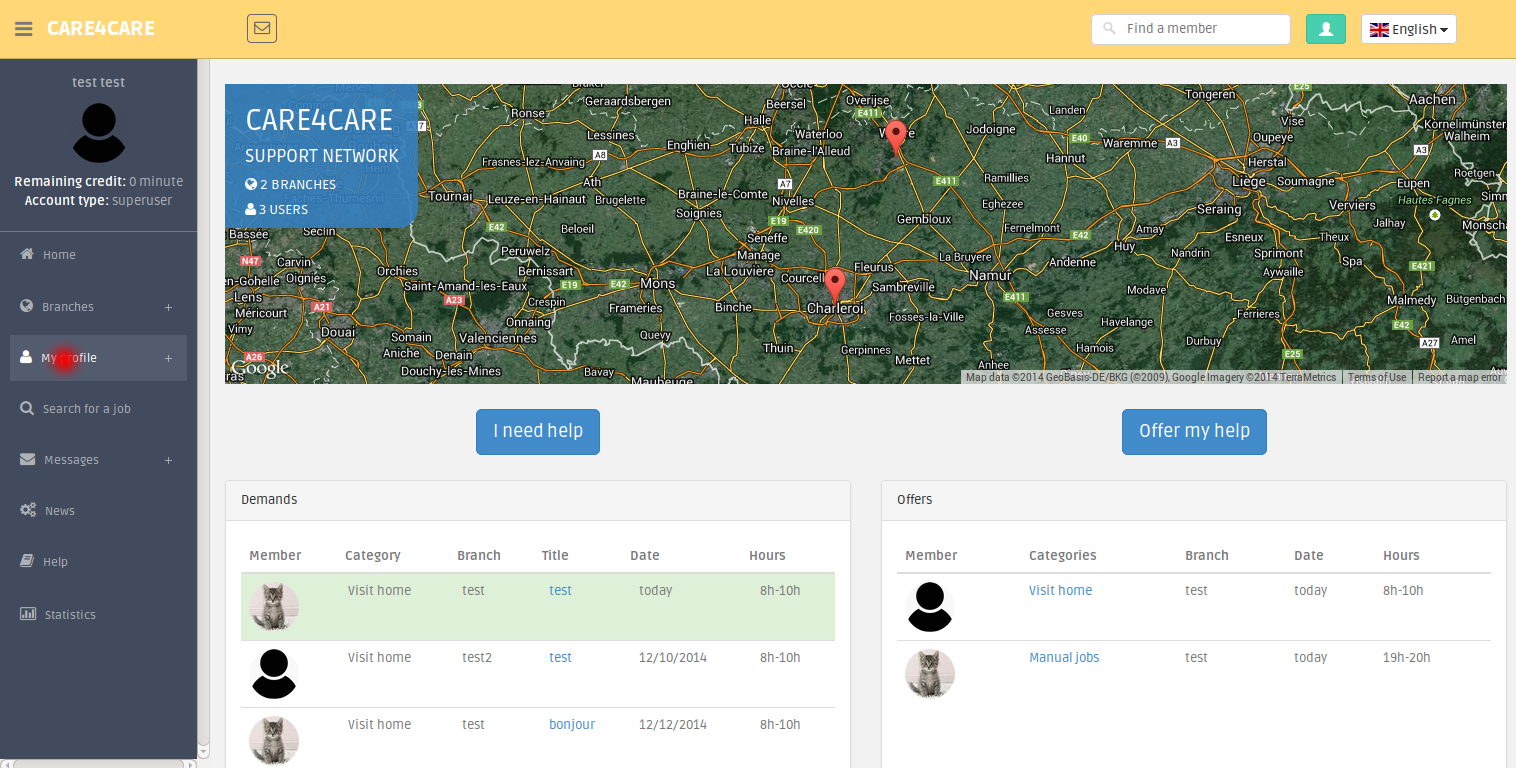
\includegraphics[width=\textwidth]{img/profil1.png}
   \caption{Display: Step 1}
\end{figure}
\begin{figure}[!ht]
   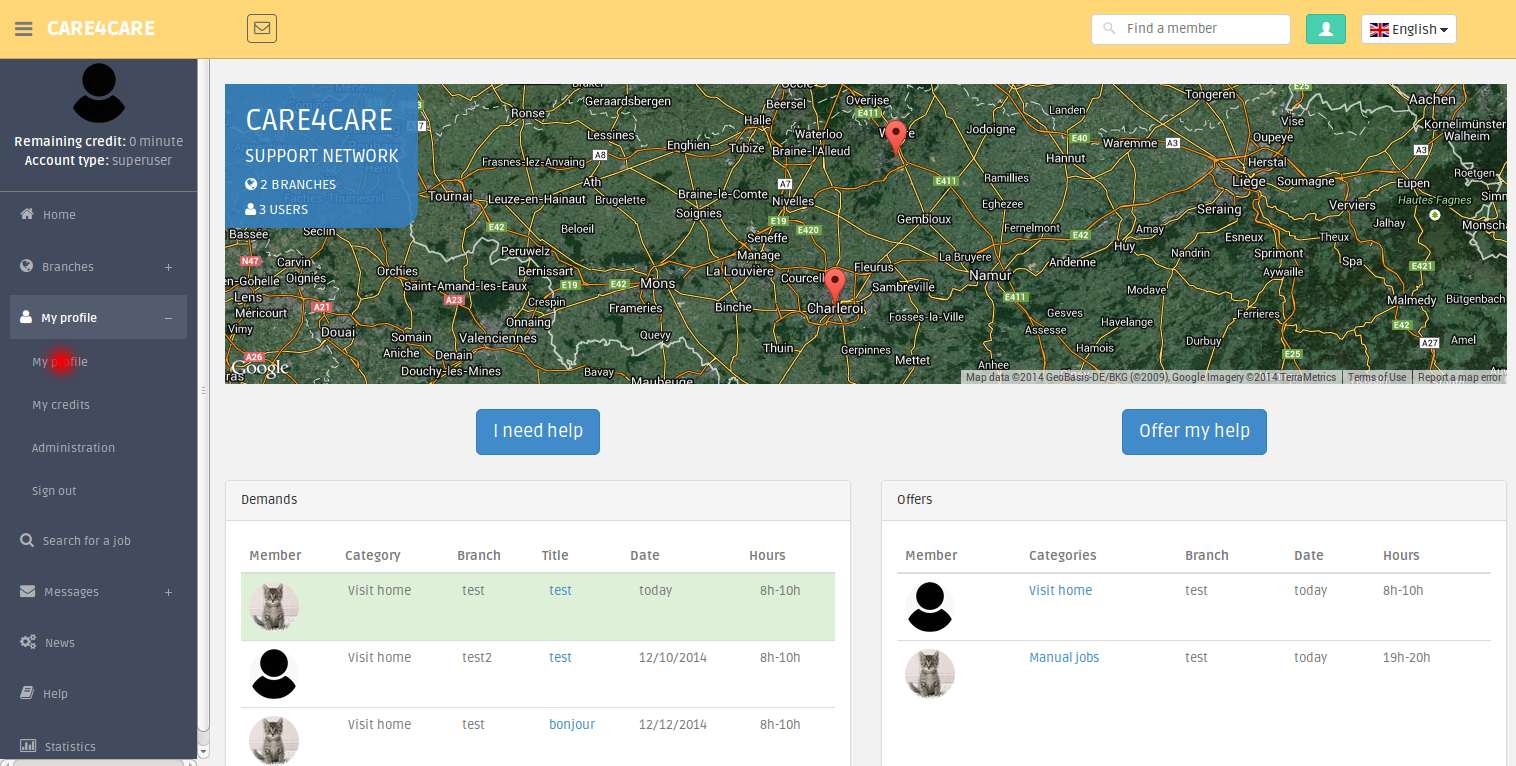
\includegraphics[width=\textwidth]{img/profil2.png}
   \caption{Display: Step 2}
\end{figure}
\begin{figure}[!ht]
   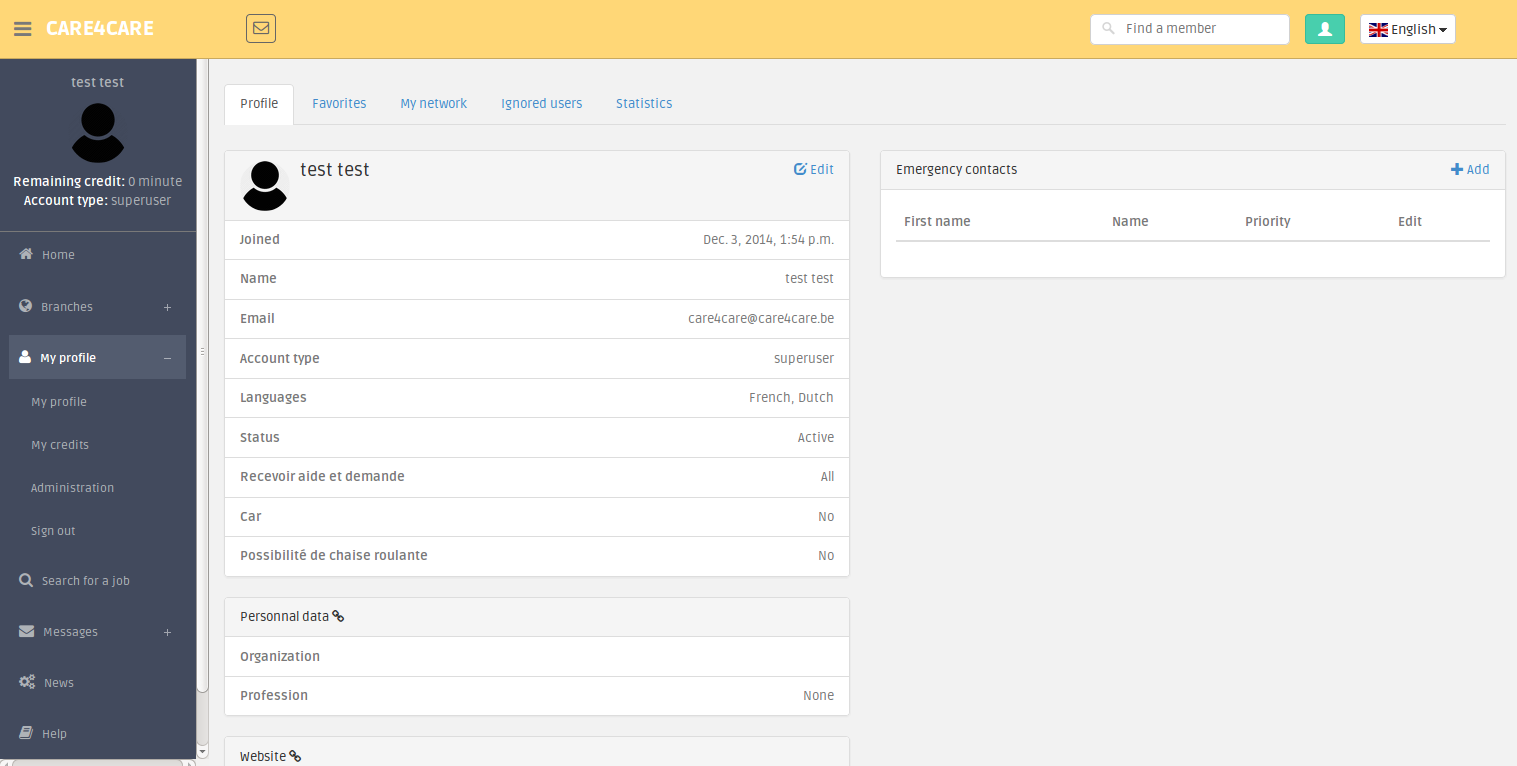
\includegraphics[width=\textwidth]{img/profil3.png}
   \caption{Display: Result}
\end{figure}

\clearpage
\subsection{Edit my profil}
Go to: \textbf{My profile}.
\begin{figure}[!ht]
   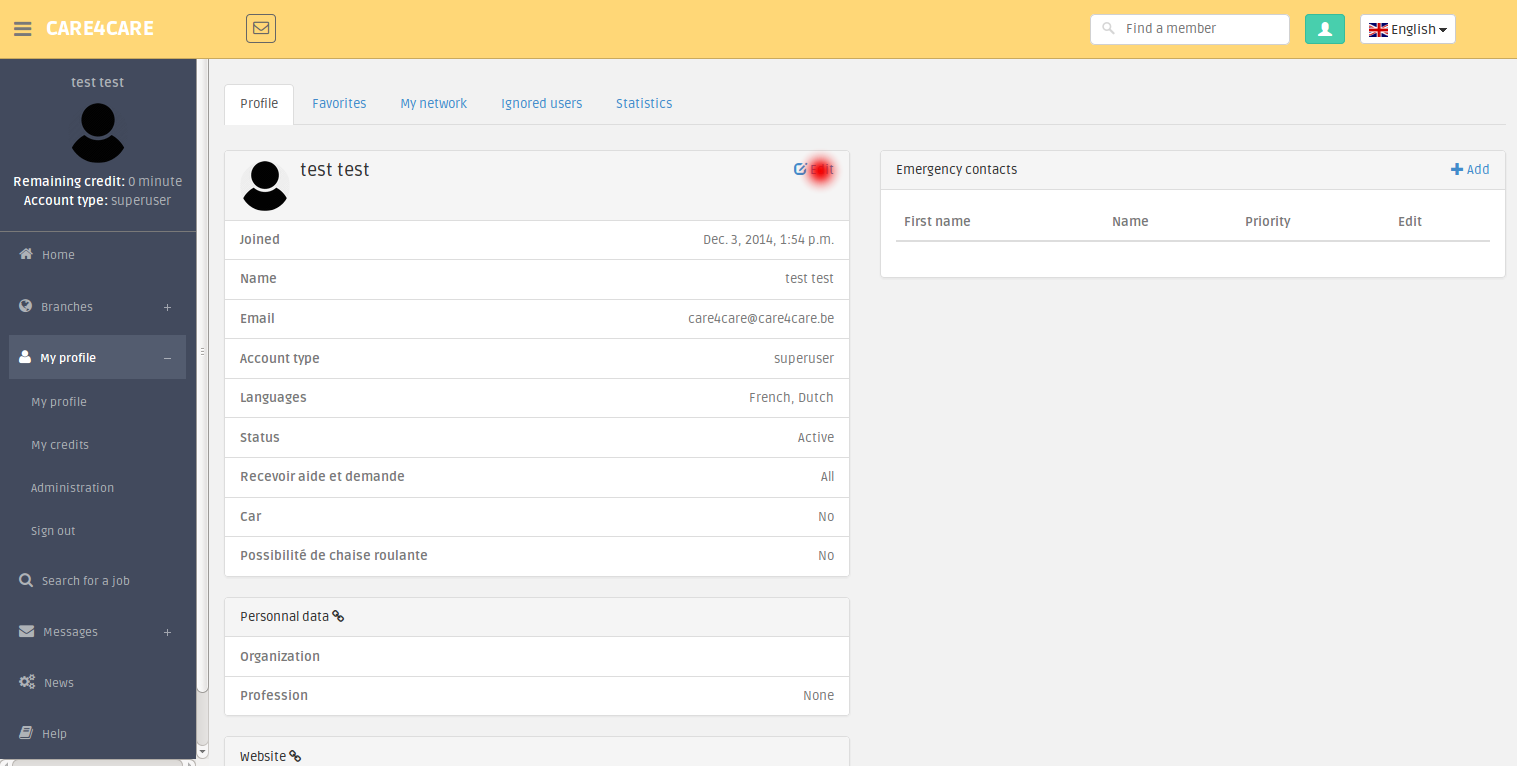
\includegraphics[width=\textwidth]{img/profil4.png}
   \caption{Edit: Step 1}
\end{figure}
\begin{figure}[!ht]
   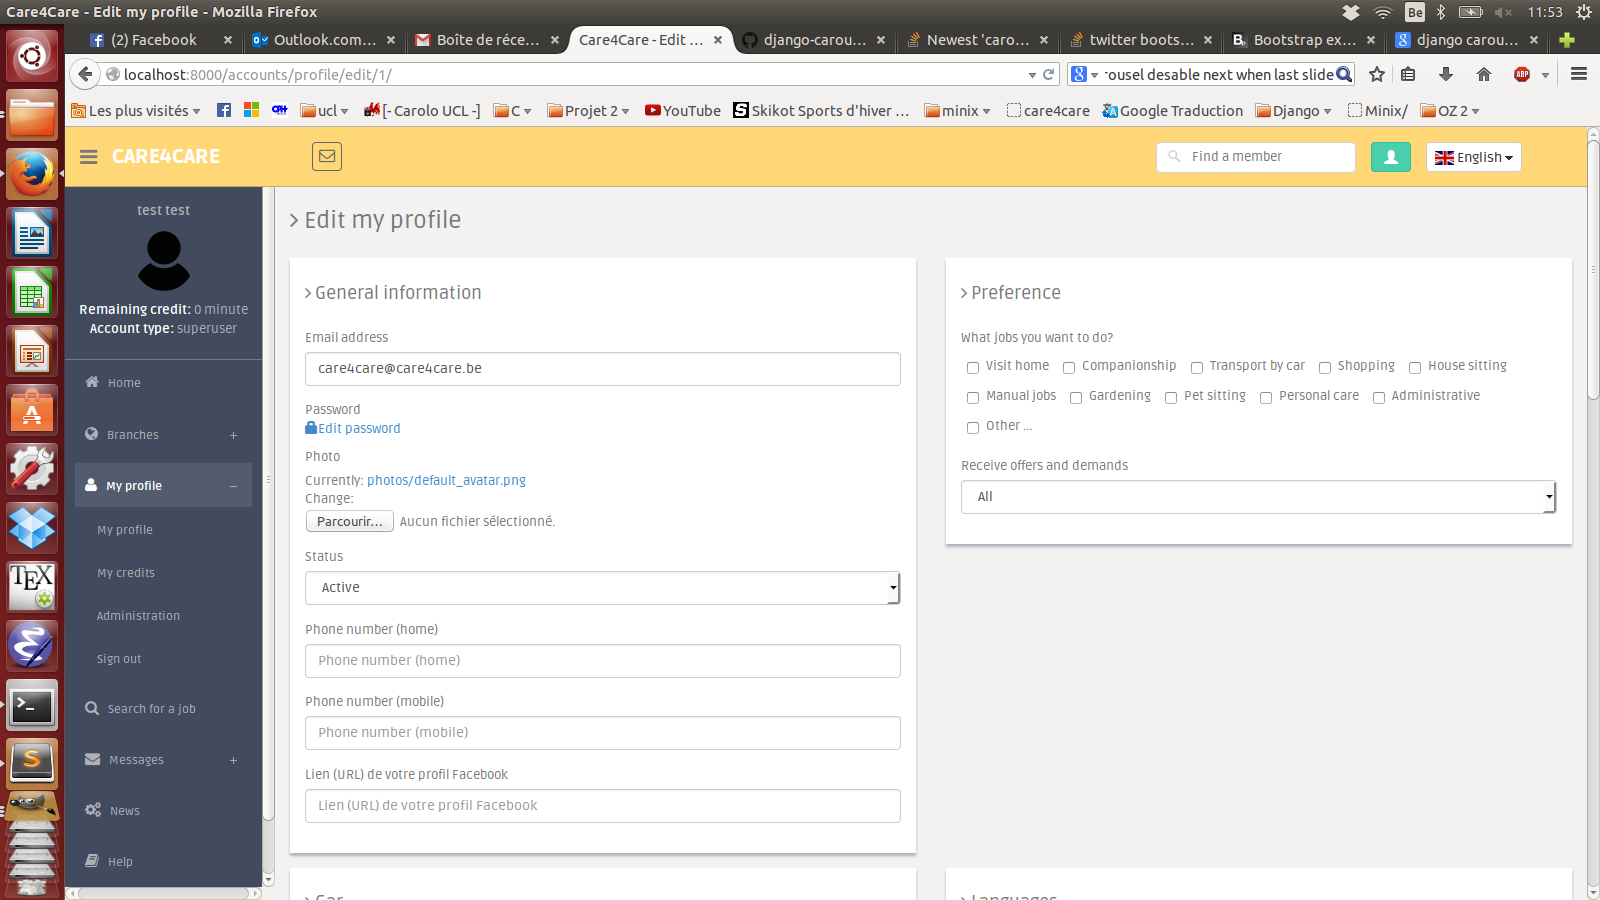
\includegraphics[width=\textwidth]{img/profil5.png}
   \caption{Edit: Step 2 - Fill in this form}
\end{figure}
\begin{figure}[!ht]
   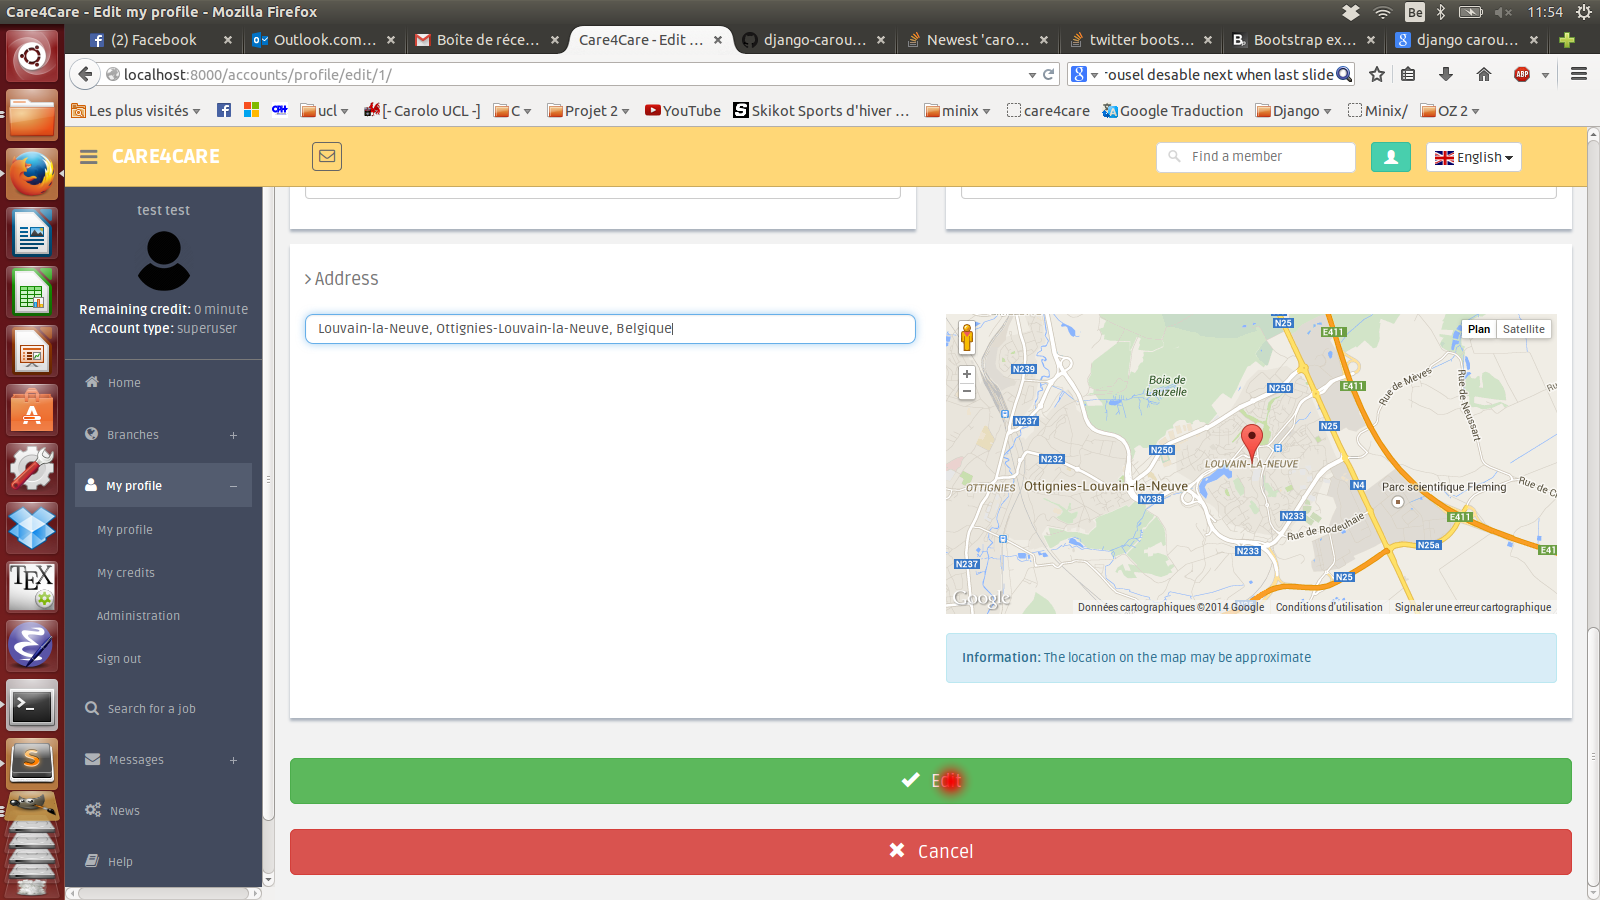
\includegraphics[width=\textwidth]{img/profil6.png}
   \caption{Edit: Step 3 - Send modifications}
\end{figure}

\clearpage
\section{Ask for help}
\begin{figure}[!ht]
   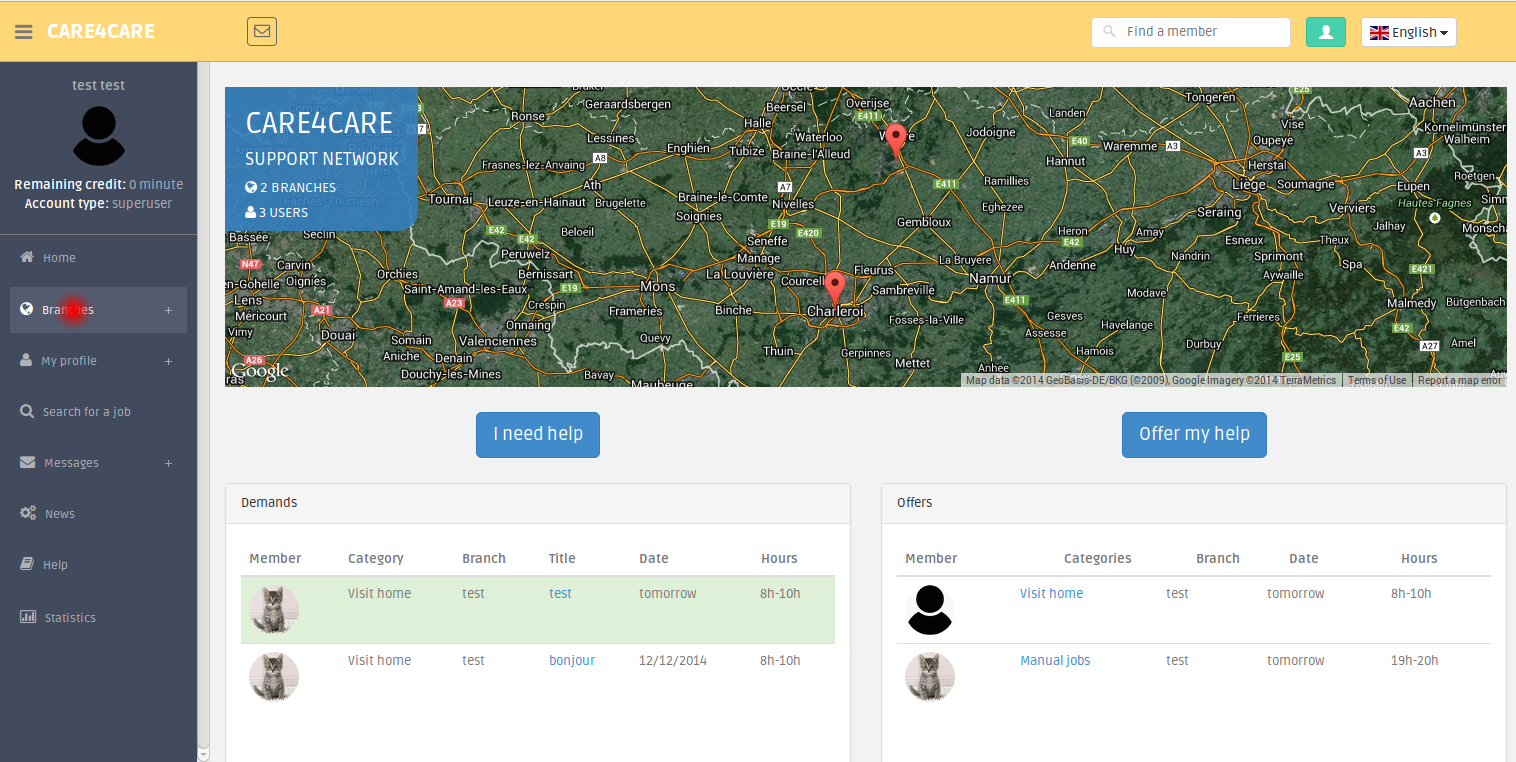
\includegraphics[width=\textwidth]{img/dem1.png}
   \caption{Ask: Step 1}
\end{figure}
\begin{figure}[!ht]
   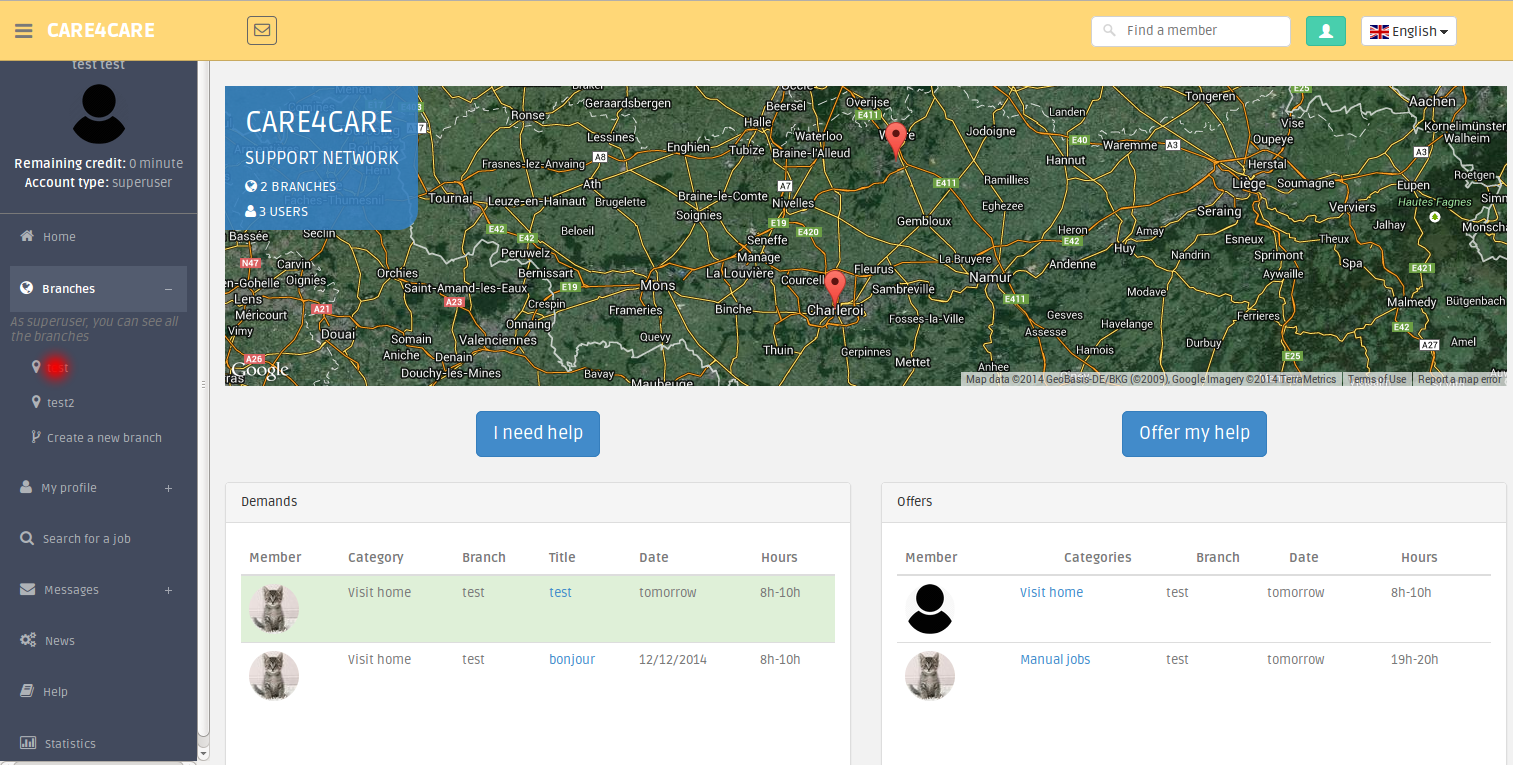
\includegraphics[width=\textwidth]{img/dem2.png}
   \caption{Ask: Step 2 - Choose a branch}
\end{figure}
\begin{figure}[!ht]
   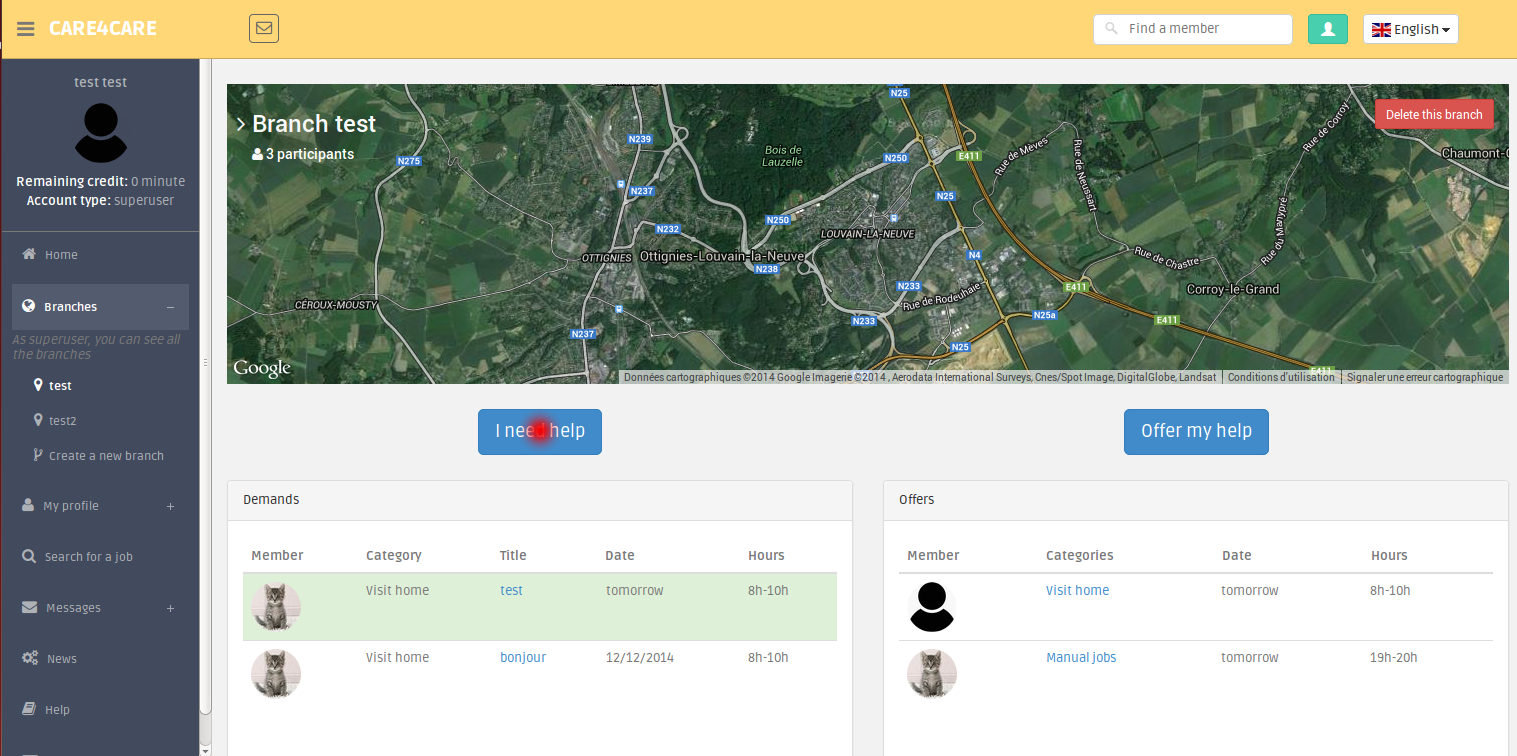
\includegraphics[width=\textwidth]{img/dem3.png}
   \caption{Ask: Step 3}
\end{figure}
\begin{figure}[!ht]
   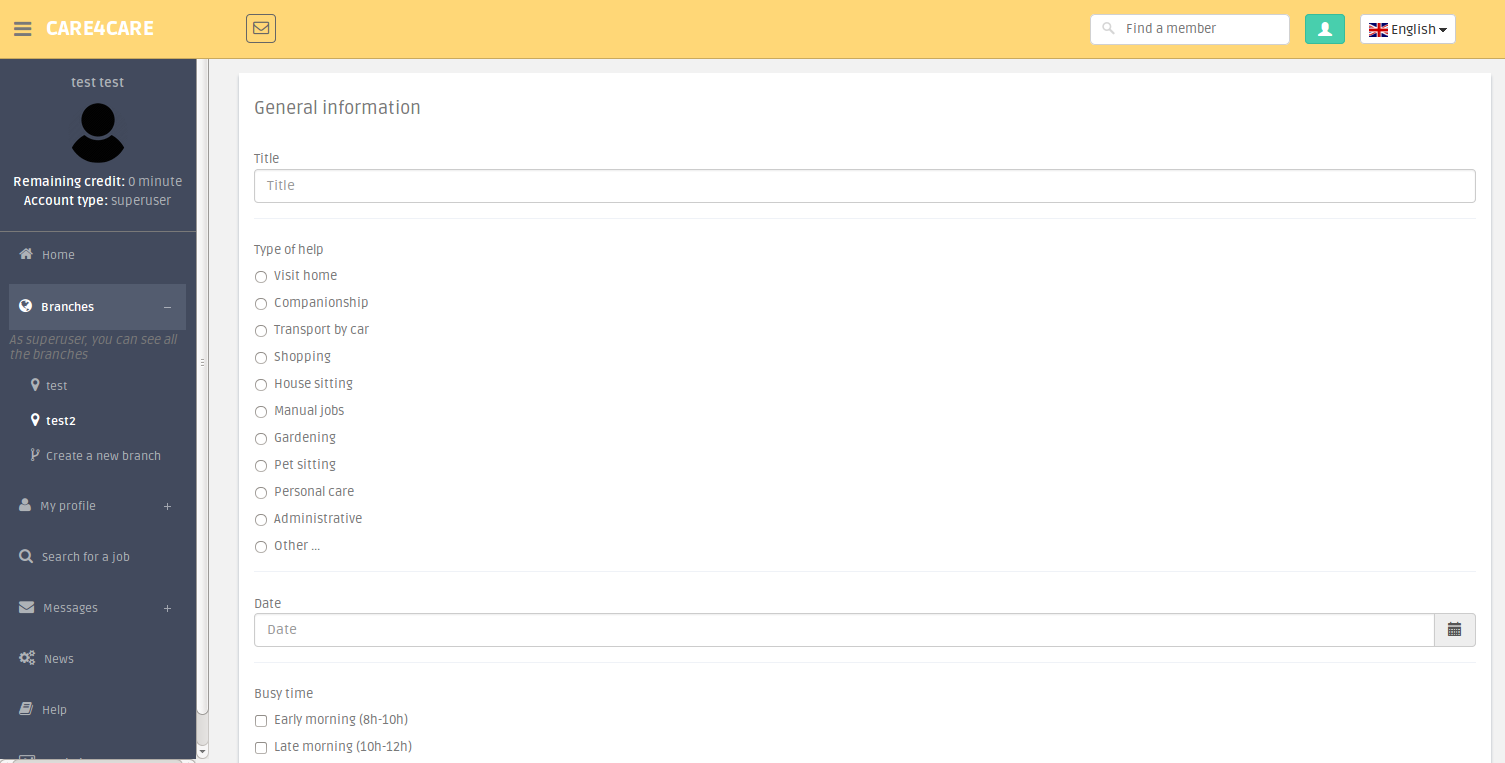
\includegraphics[width=\textwidth]{img/dem4.png}
   \caption{Ask: Step 4 - Fill in this form}
\end{figure}
\begin{figure}[!ht]
   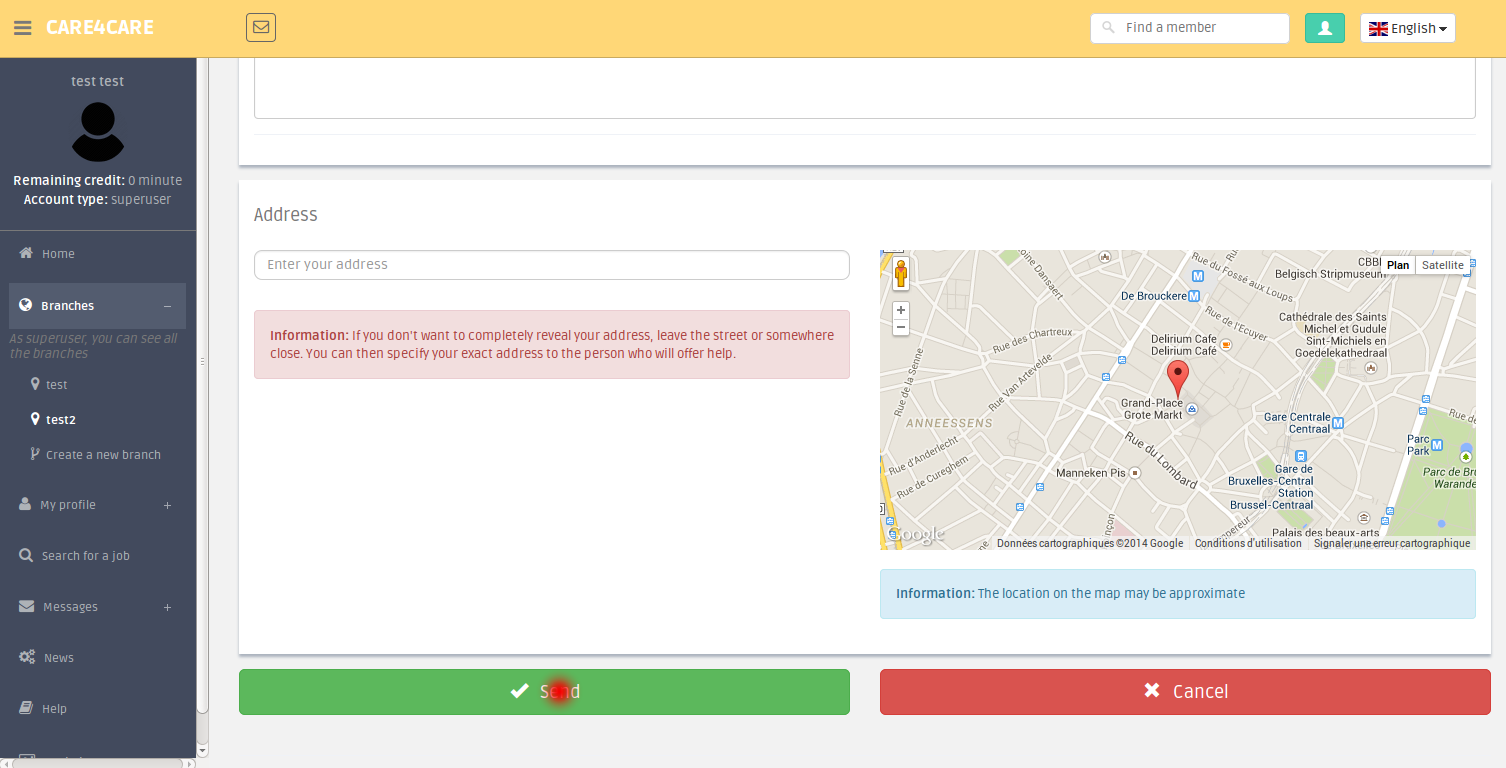
\includegraphics[width=\textwidth]{img/dem5.png}
   \caption{Ask: Step 5 - Send demand}
\end{figure}

\clearpage
\section{Offer my help}
Follow the same steps for \textbf{Ask for help} but click on \textbf{Offer my help} instead of I need help.


\section{Favorites and My network}
\subsection{What are the differences?}
You can do demands addressed only to people in \textbf{Favorites}.
People in \textbf{My network} will see more information about you.
\subsection{How to add people in Favorites?}
Go to: \textbf{My profile}.
\begin{figure}[!ht]
   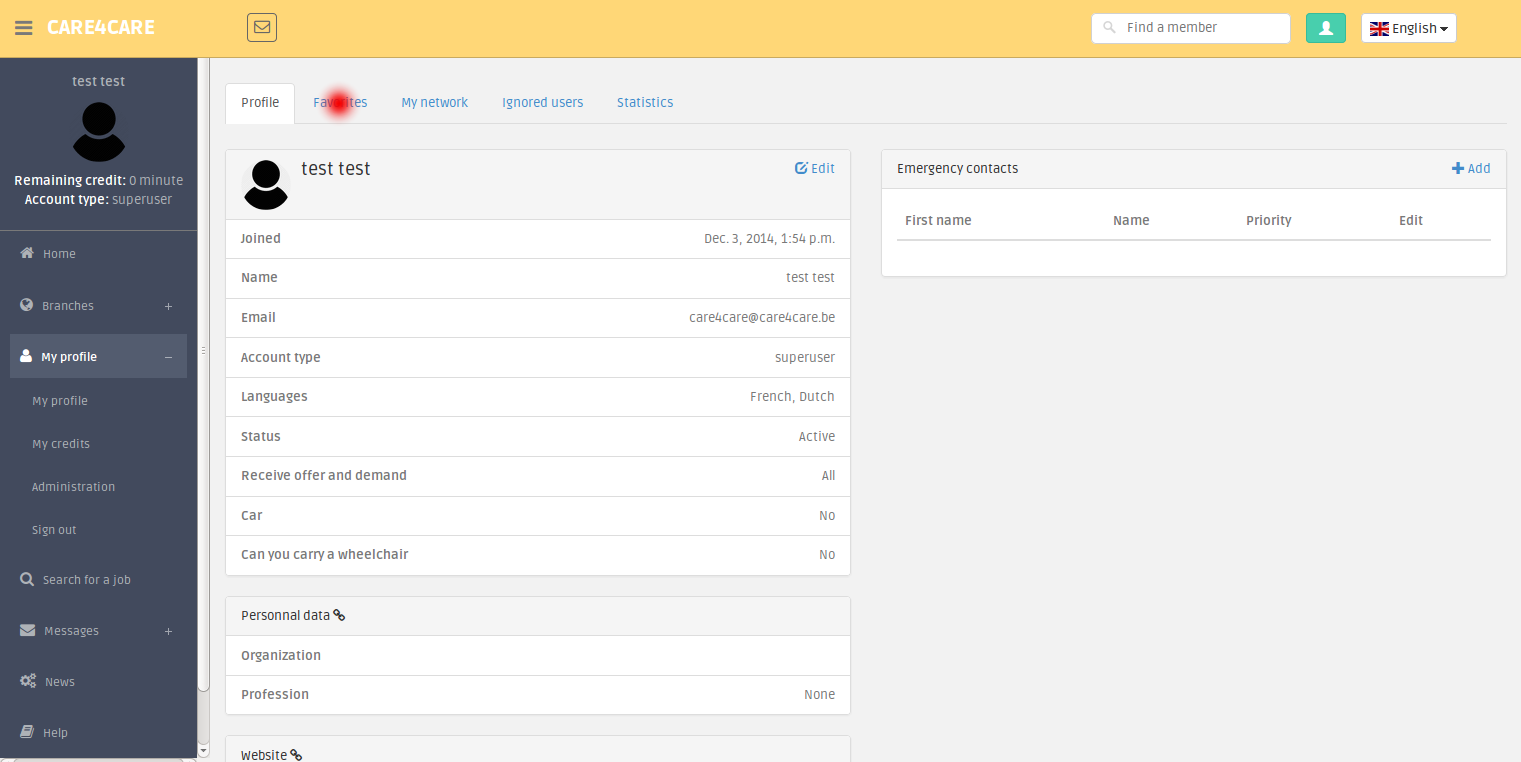
\includegraphics[width=\textwidth]{img/fav1.png}
   \caption{Favorites: Step 1}
\end{figure}
\begin{figure}[!ht]
   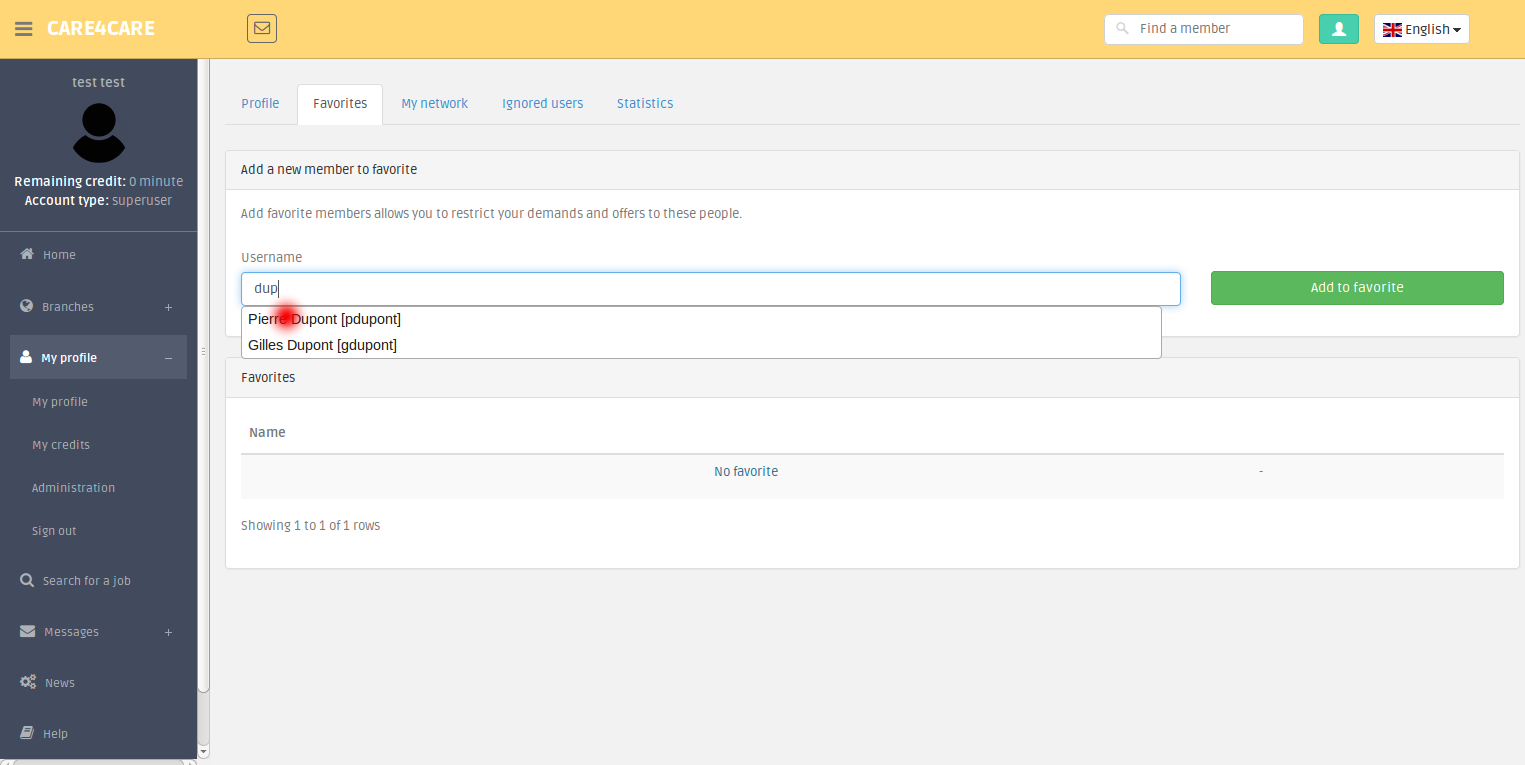
\includegraphics[width=\textwidth]{img/fav2.png}
   \caption{Favorites: Step 2 - Fill the field and select the user}
\end{figure}
\begin{figure}[!ht]
   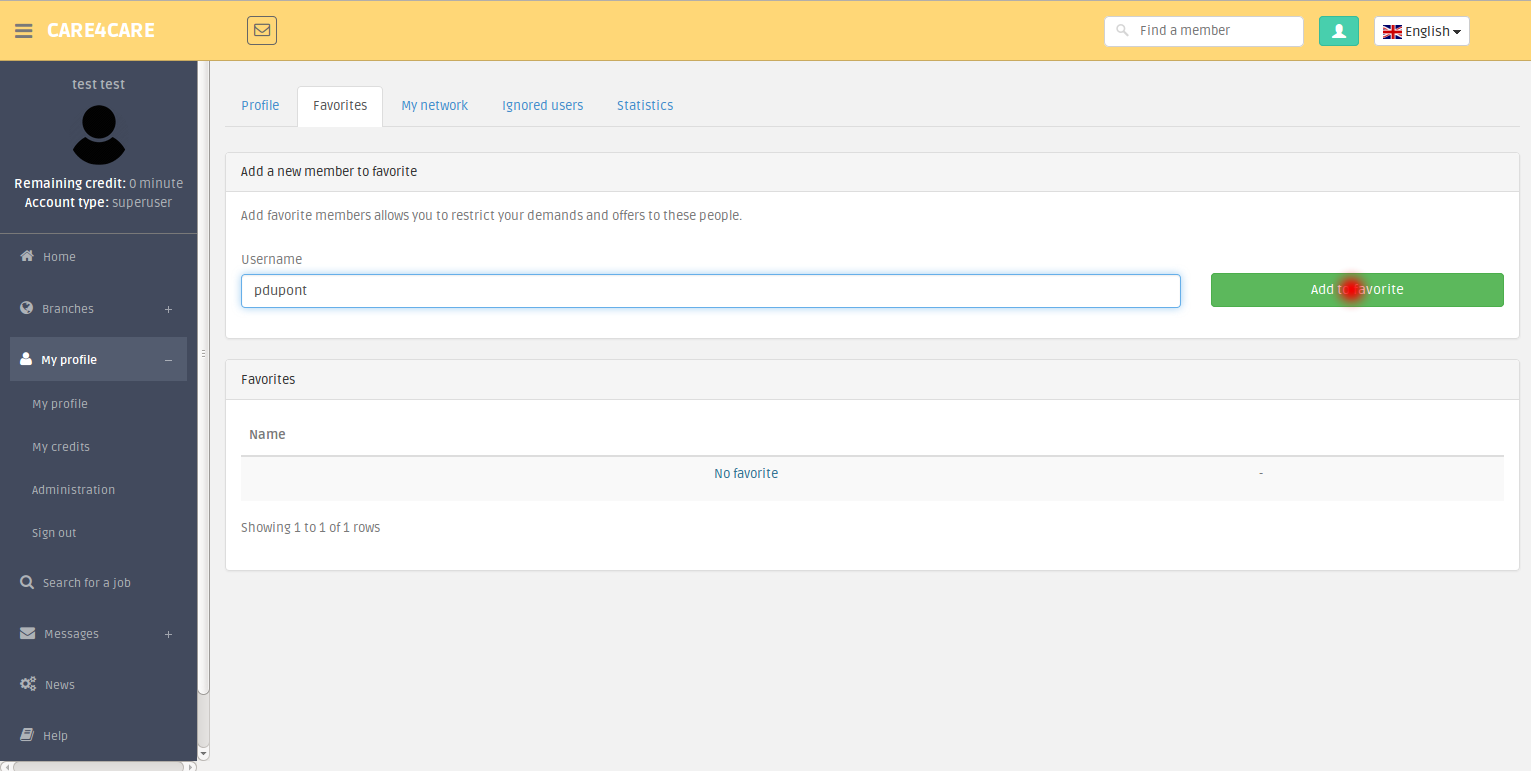
\includegraphics[width=\textwidth]{img/fav3.png}
   \caption{Favorites: Step 3}
\end{figure}
\begin{figure}[!ht]
   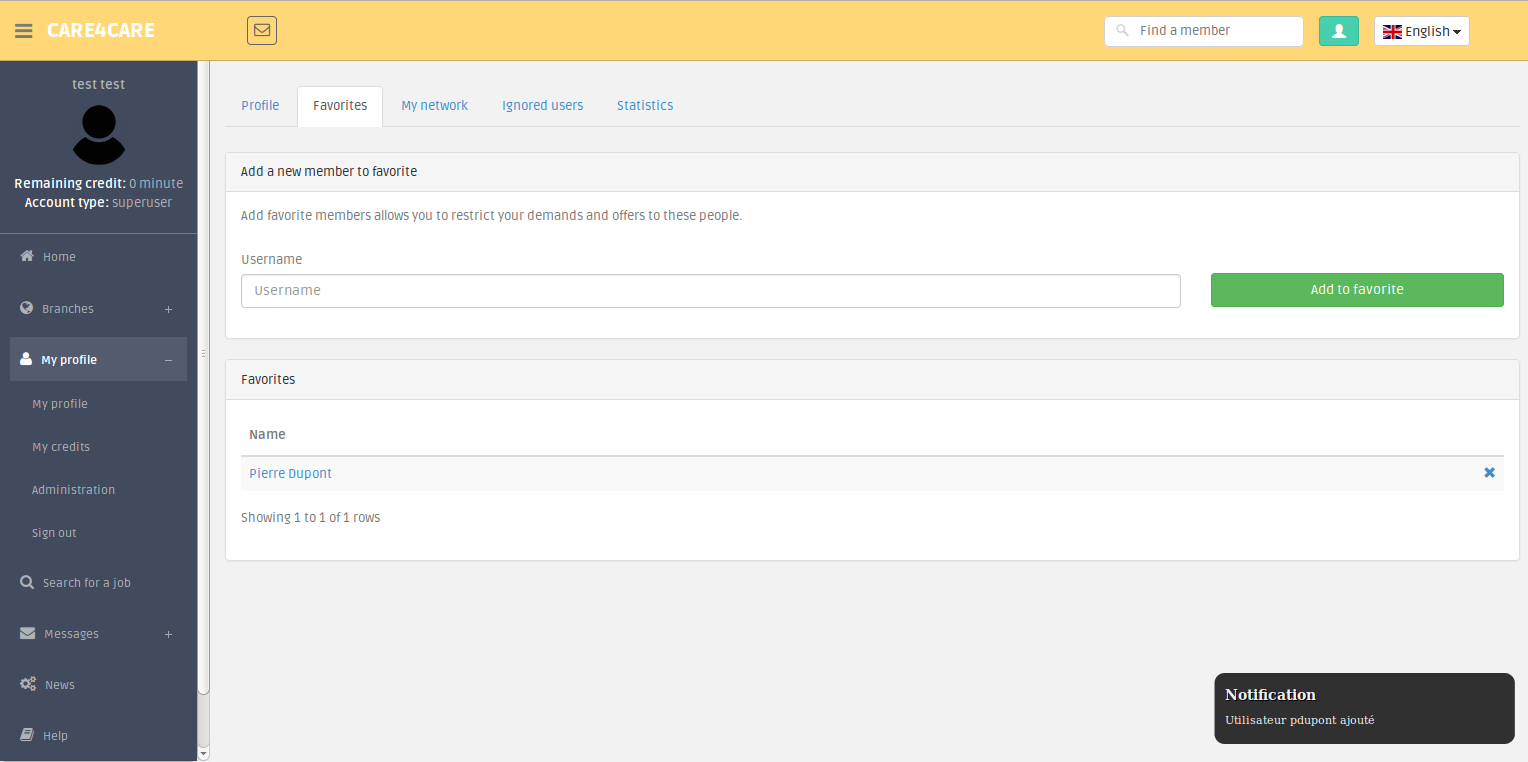
\includegraphics[width=\textwidth]{img/fav4.png}
   \caption{Favorites: Result}
\end{figure}
\subsection{How to add poeple in My network}
Follow the same steps as favorites but first click \textbf{My network} instead of \textbf{Favorites}.

\clearpage
\section{Messages}
Click on the small mailbox beside \textbf{Care4Care} or click on \textbf{Messages} in the menu, then choose, for example, \textbf{Inbox} , will lead you to the same page. 
\subsection{Read a received message}
\begin{figure}[!ht]
   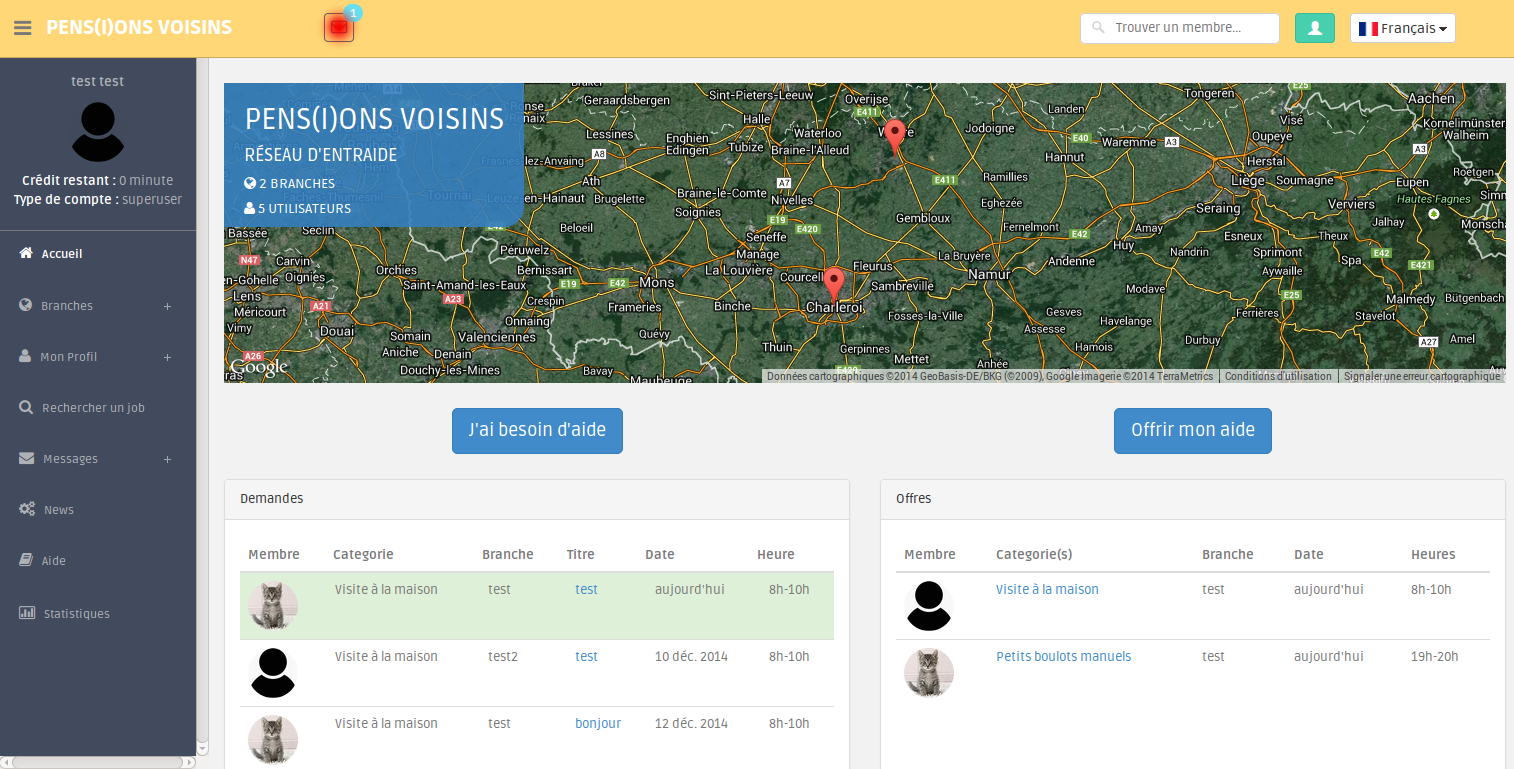
\includegraphics[width=\textwidth]{img/mess1.png}
   \caption{Message: Step 1}
\end{figure}
\begin{figure}[!ht]
   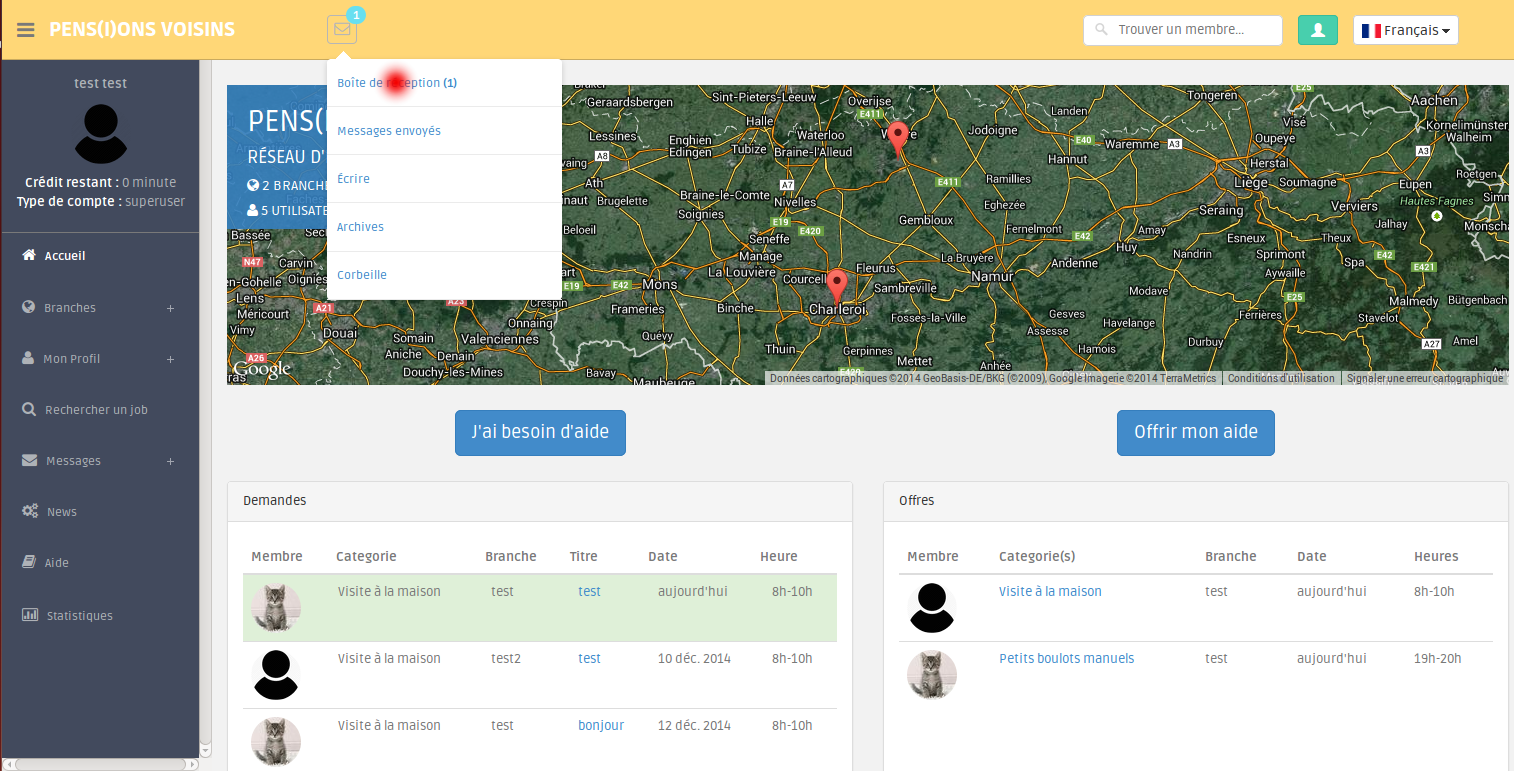
\includegraphics[width=\textwidth]{img/mess2.png}
   \caption{Message: Step 2}
\end{figure}
\begin{figure}[!ht]
   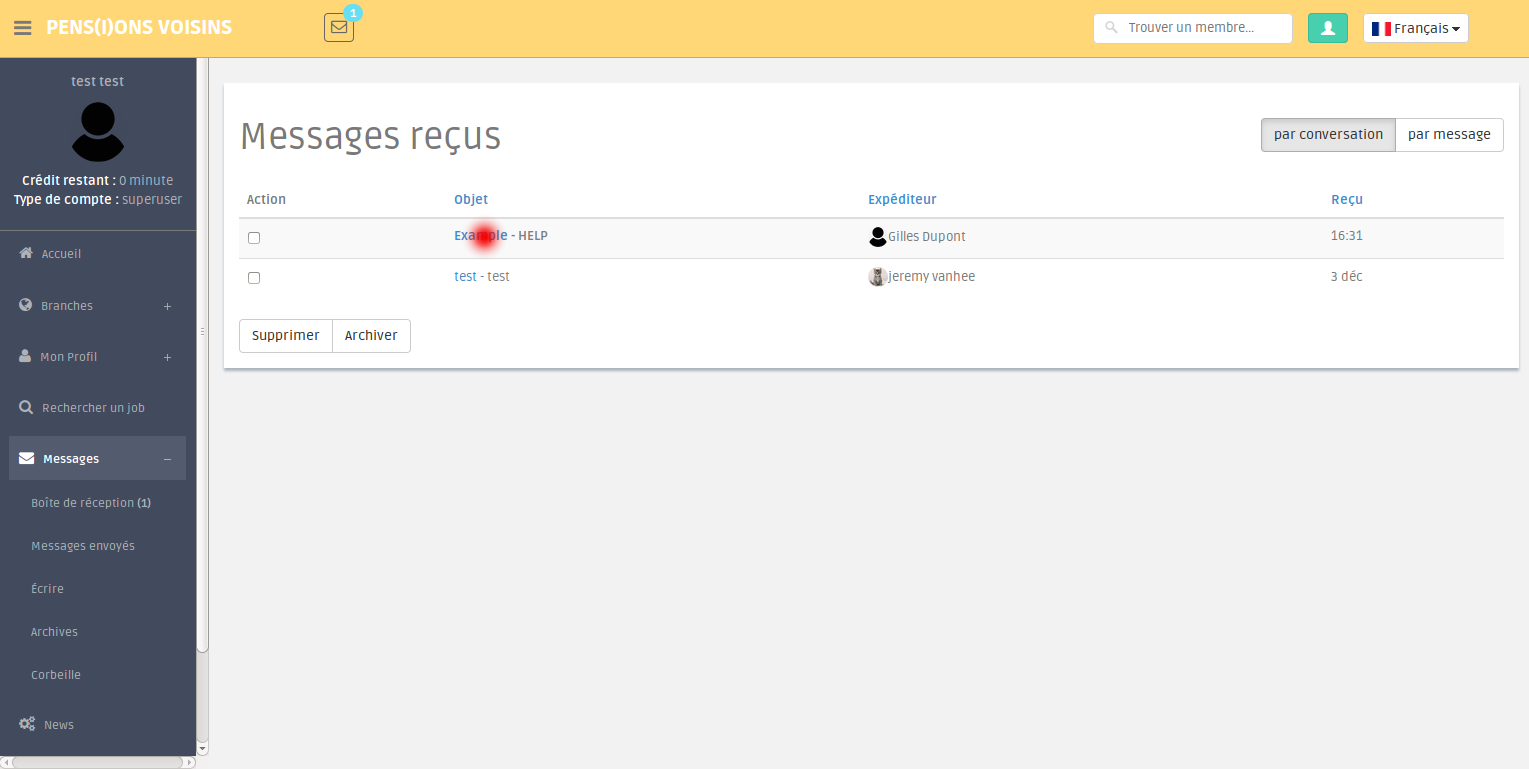
\includegraphics[width=\textwidth]{img/mess3.png}
   \caption{Message: Step 3}
\end{figure}
\begin{figure}[!ht]
   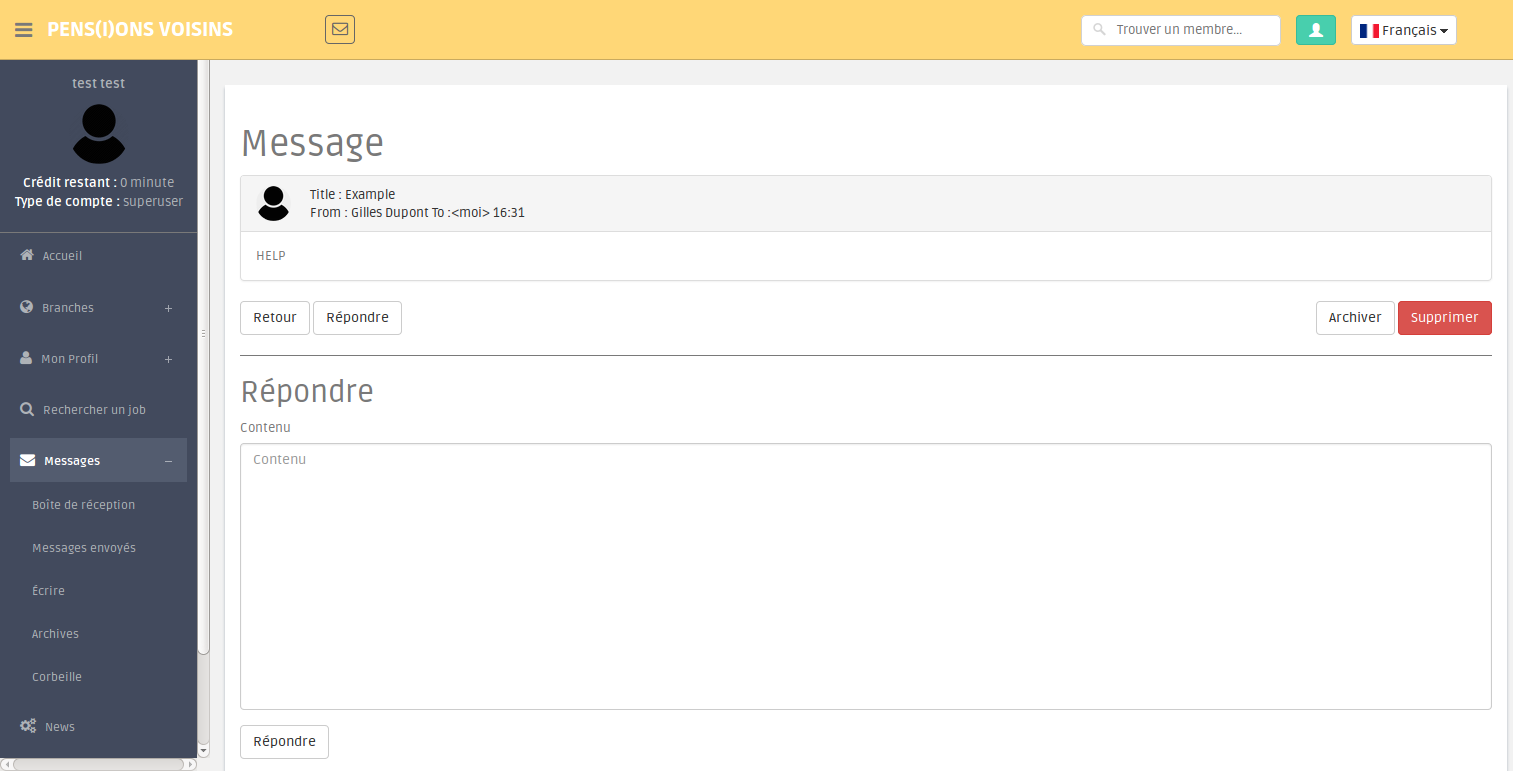
\includegraphics[width=\textwidth]{img/mess4.png}
   \caption{Message: Result}
\end{figure}


\end{document}